\quad \quad Миний хувьд дадлагын явцад хөгжүүлсэн 2 төслийн нэг нь \textbf{"Khuur"} буюу морин хуур хөглөх болон морин хуур анхлан суралцагчдад зориулсан видео хичээлүүд агуулсан аппликейшн юм. "Khuur"-ийн анхны хувилбарт зөвхөн морин хуур хөглөх үйлдэл шаардлагатай байсан учир видео хичээлийн хэсгийг түр хугацаанд хойшлуулсан болно. Харин 2 дахь нь монгол мөнгөн дэвсгэртийн дата зураг цуглуулах flutter аппликейшн юм. Энэ апп нь AWS технологи ашиглан хэрэглэгчдээ бүртгэж, зурган дата хадгалж ХандПро компаний хөгжүүлж буй машин сургалтын модельд ашиглагдана. Мөн уг аппликейшнийг зарим нэг дэлгүүрээр тарааж дата цуглуулаад эхэлсэн билээ.
\section{Хэрэглэгчийн шаардлага}
    \subsection{Khuur апп}
        \subsubsection{Функциональ хэрэглэгчийн шаардлагууд}
         \begin{itemize}
            \item Хэрэглэгч нэвтрэх шаардлагагүй байх
            \item Хэрэглэгч анх ороход морин хуур хөглөх хэсгийг харуулдаг байх
            \item Апп нь гар утасны микрофоны тусламжтайгаар морин хуурын дугаралтыг сонсдог байх 
            \item Дэлгэц дээр морин хуурын зураг болон давтамжийн анализын үр дүнг харуулдаг байх
            \item Апп нь "real-time"-аар хөгжмийн давтамжийг анализ хийдэг байх
            \item Апп нь хэрэглэгчид давтамжийн анализаас хамаарч зөвлөх мэдээллийг будагдсан суман тэмдэг ашиглан харуулдаг байх (жишээ нь, шар баруун эргүүлэх тэмдэг, улаан зүүн эргүүлэх тэмдэг) 
            \item Хэрэглэгч 440, 442 герцийн сонголттойгоор хөглөх боломжтой байна
            \item Хэрэглэгч автомат болон автомат бус горимын сонголттой байна
            \item автомат горим нь автоматаар аль ноотыг хөглөж байгааг олж анализ хийнэ 
            \item Автомат бус горим нь хэрэглэгчийн сонгосон си эсвэл фа ноотын аль нэгийн давтамжийг л анализ хийнэ
            \item Апп нь морин хуурын хичээлийн хэсэгтэй байх
            \item Апп нь хичээлүүдийн жагсаалтыг харуулдаг байх
            \item Хичээлүүд нь видео контент болон бичгэн байдлаар хосолсон байх
        \end{itemize}
      \subsubsection{Функциональ бус шаардлага}
        \begin{itemize}
            \item Апп нь хэрэглэхэд хялбар ойлгомжтой дизайнтай байх
            \item Responsive дизайнтай байх
            \item Апп нь Fast Fourier Transform (FFT) ашиглан хөгжмийн давтамжийг тодорхойлно
            \item Давтамжийн анализыг 60FPS хурдны давтамжтайгаар гүйцэтгэх
            \item Системийг бага CPU болон Memory ашиглах байдлаар хөгжүүлэх
            \item Flutter дээрх оптимацлах аргуудыг ашиглах
            \item Системд алдаа гарсан тохиолдолд, хэрэглэгчид заавал мэдэгдэнэ.
            \item Системийн хэрэглэгчийн интерфейс дээр ашиглах товч(button), тект, гарчигууд нэг хэв загвартай байна
            \item Апп нь Android болон IOS гар утсан дээр алдаагүй ажилдаг байх
            \item Апп нь дараа дараагийн шинэчлэлтүүдтэй зохицож ажилдаг байх
        \end{itemize}
    \subsection{Data spider апп}
        \subsubsection{Функциональ хэрэглэгчийн шаардлагууд}
             \begin{itemize}
                \item Аппруу анх ороход нэвтрэх хуудсыг харуулдаг байх
                \item Хэрэглэгч шинэ нэвтрэлт үүсгэнэ эсвэл бүртгүүлсэн нэвтрэх нэр болон нууц үгийг ашиглан нэвтрэх боломжтой байх
                \item Апп нь зааврын хэсэгтэй байх
                \item Апп нь гар утасны камер нээх эрхтэй байна
                \item Хэрэглэгч мөнгөн дэвсгэртийн урд болон ар талын зургийг авах боломжтой байна
                \item Хэрэглэгч зургийг нь авсан мөнгөн дэвсгэртийн нэмэлт мэдээллийг оруулдаг байна
                \item 50-20,000 төгрөг хүртэлх мөнгөн дэвсгэртээс сонгох боломжтой байна
                \item Дэвсгэрт болгоны тоо хэмжээг оруулдаг байна
                \item Бэлэн болсон мэдээллээ илгээж хэрэглэгчид мэдэгддэг байх
            \end{itemize}
        \subsubsection{Функциональ бус шаардлага}
            \begin{itemize}
                \item Апп нь хэрэглэхэд ойлгомжтой дизайнтай байх
                \item Зураг авахад 300ms-ээс хэтрэхгүй байх
                \item AWS Api Gateway, Lambda, DynamoDB, S3 ашиглан back-end шийдлийг гаргасан байх
                \item Алдаа гарсан тохиолдолд хэрэглэгчид мэдээлэлдэг байх
            \end{itemize}
\pagebreak
\section{Кhuur Use Case диаграм}
\begin{figure}[h]
	\centering
	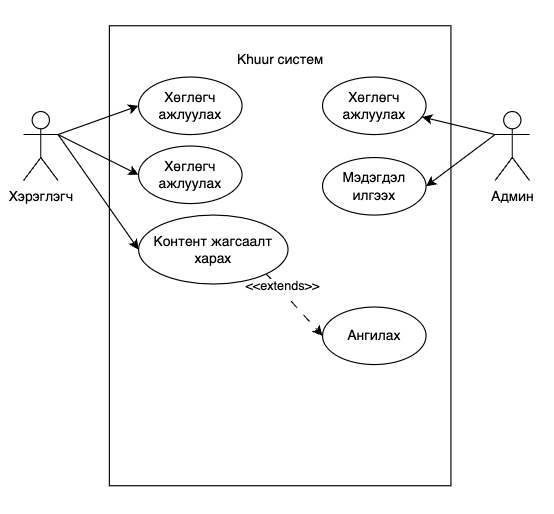
\includegraphics[width=13cm]{images/khuur-usecase.png}
	\caption{Khuur Use Case диаграм}
	\label{fig:form}
\end{figure}
\section{Data Spider Use Case диаграм}
\begin{figure}[h]
	\centering
	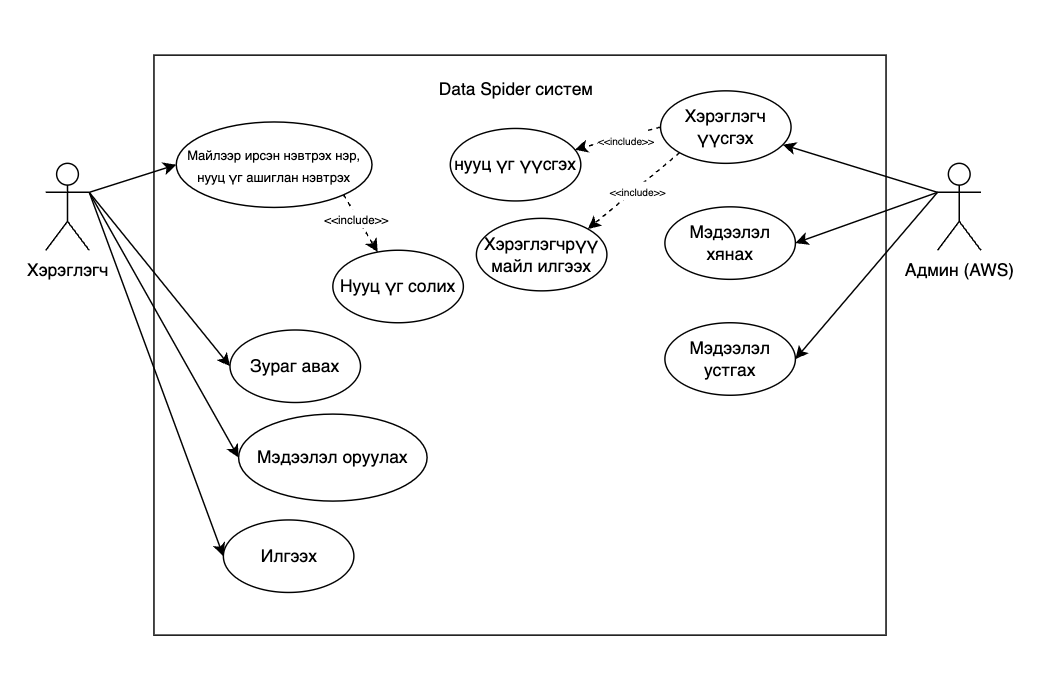
\includegraphics[width=13cm]{images/dataspider-usecase.png}
	\caption{Data Spider Use Case диаграм}
	\label{fig:form}
\end{figure}
